\documentclass{article}
\usepackage[margin=1in]{geometry}
\usepackage{amsmath}
\usepackage{amssymb}
\usepackage{amsthm}
\usepackage{bm}
\usepackage{hyperref}
\usepackage{graphicx}
\usepackage{caption}
\usepackage{listings}
\usepackage{xcolor}
\usepackage{float}
\usepackage{booktabs}
\usepackage{longtable}
\usepackage{multirow}
\usepackage{placeins}
\graphicspath{{figures/}}

% Code style
\lstdefinestyle{code}{
  basicstyle=\ttfamily\small,
  numbers=left,
  numberstyle=\tiny,
  numbersep=8pt,
  keywordstyle=\color{blue},
  commentstyle=\color{teal!70!black},
  stringstyle=\color{orange!70!black},
  showstringspaces=false,
  breaklines=true,
  frame=single,
  framerule=0.3pt,
  rulecolor=\color{black!15}
}
\lstset{style=code}

\title{Prompt Engineering Playbook: From Zero-Shot Patterns to Automated Optimization}
\author{}
\date{\today}

\begin{document}
\maketitle

\section{Zero-shot, Few-shot, and Chain-of-Thought}
\subsection{Progressive prompting modes}
Prompting strategies evolve from minimal instructions to structured reasoning. Zero-shot leverages pretrained priors without examples; few-shot embeds demonstrations; Chain-of-Thought (CoT) encourages explicit intermediate reasoning. Figure~\ref{fig:prompt_modes_en} illustrates the progression of these modes toward controlled verification.
\begin{figure}[H]
  \centering
  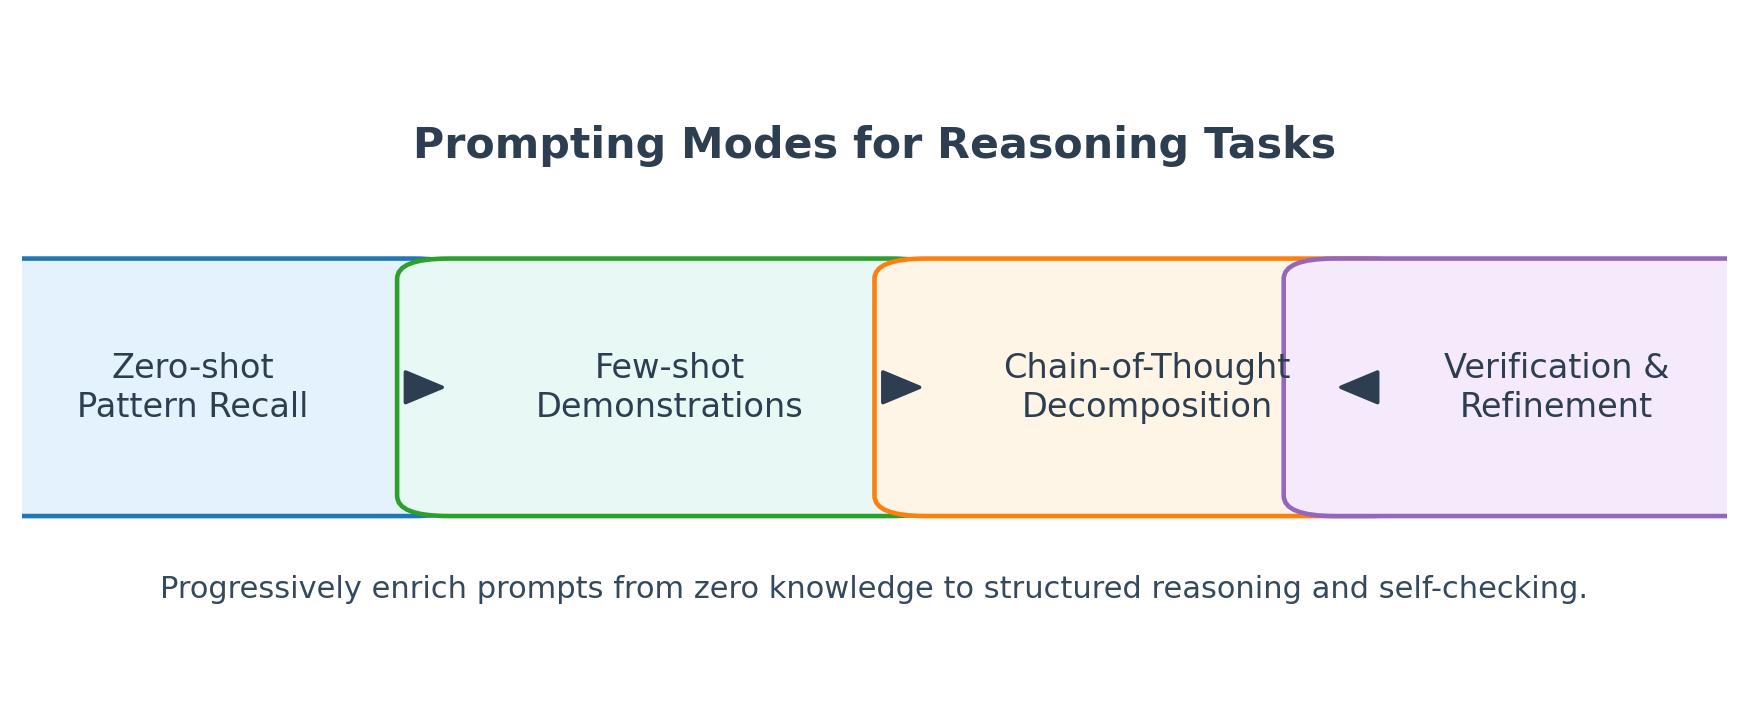
\includegraphics[width=0.92\textwidth]{prompt_modes.png}
  \caption{Prompting modes: enriching instructions from zero-shot to few-shot and Chain-of-Thought with verification.}
  \label{fig:prompt_modes_en}
\end{figure}

\subsection{Zero-shot guidelines}
\begin{itemize}
  \item \textbf{Instruction clarity:} Specify the task, desired medium, and output constraints (e.g., “Summarize in Chinese with three bullet points”).
  \item \textbf{Role and guardrails:} Define behavior via system prompts such as “You are a cybersecurity analyst who must provide factual assessments only.”
  \item \textbf{Semantic anchors:} Provide keywords, timeframes, or domain hints to narrow interpretation.
\end{itemize}
Zero-shot works for direct Q\&A or classification, yet struggles on multi-step reasoning without additional scaffolding.

\subsection{Constructing few-shot exemplars}
\begin{itemize}
  \item \textbf{Representative coverage:} Include diverse classes and edge cases while keeping format consistent.
  \item \textbf{Alignment:} Mirror input/output templates—JSON schemas, Markdown tables, structured lists.
  \item \textbf{Ordering:} Place the most critical example first to bias the model toward the desired pattern.
  \item \textbf{Counterexamples:} For complex domains, show incorrect attempts alongside corrected answers to prime error detection.
\end{itemize}

\subsection{Chain-of-Thought prompting}
CoT prompts request that the model explain its reasoning before answering:
\begin{itemize}
  \item \textbf{Template scaffold:} Adopt “Problem → Analysis → Answer” patterns or instruct “Let’s reason step-by-step.”
  \item \textbf{Decomposition:} Break down arithmetic, logic, or planning problems into subgoals, enabling the model to use intermediate variables.
  \item \textbf{Verification:} Pair with self-consistency sampling or separate verifier models to reject incoherent chains.
\end{itemize}
In production, choose low temperature for determinism, or combine with beam search to explore multiple chains before selecting a consensus answer.

\section{ReAct (Reason + Act) and Tree-of-Thoughts}
\subsection{ReAct workflow}
ReAct alternates between reasoning statements and tool invocations. The agent produces a \texttt{Thought}, optionally issues an \texttt{Action} calling a tool, receives an \texttt{Observation}, and repeats until a \texttt{Final Answer} is available. Integration tips:
\begin{enumerate}
  \item Enumerate available tools, their input schema, and usage limits within the prompt.
  \item Limit loop iterations, detect repeated queries, and penalize redundant actions.
  \item Log all thought/action traces for auditability and post-hoc debugging.
\end{enumerate}

\subsection{Tree-of-Thoughts reasoning}
Tree-of-Thoughts (ToT) expands search into a decision tree where each node is a partial reasoning path:
\begin{itemize}
  \item \textbf{Generation policy:} Produce several candidate thoughts per depth via breadth-first, depth-first, or MCTS-style exploration.
  \item \textbf{Evaluators:} Score nodes with separate heuristics or models (reward models, constraint checkers) and retain promising branches.
  \item \textbf{Pruning:} Cull low-scoring branches to stay within token and latency budgets.
\end{itemize}
ToT excels at math, planning, and program repair where multiple alternative paths must be considered before selecting the best outcome.

\subsection{Integrated reasoning stack}
Figure~\ref{fig:reasoning_stack_en} shows how system prompts, memory buffers, ReAct loops, ToT planners, tool use, and evaluators interact in a full-stack prompting architecture.
\begin{figure}[H]
  \centering
  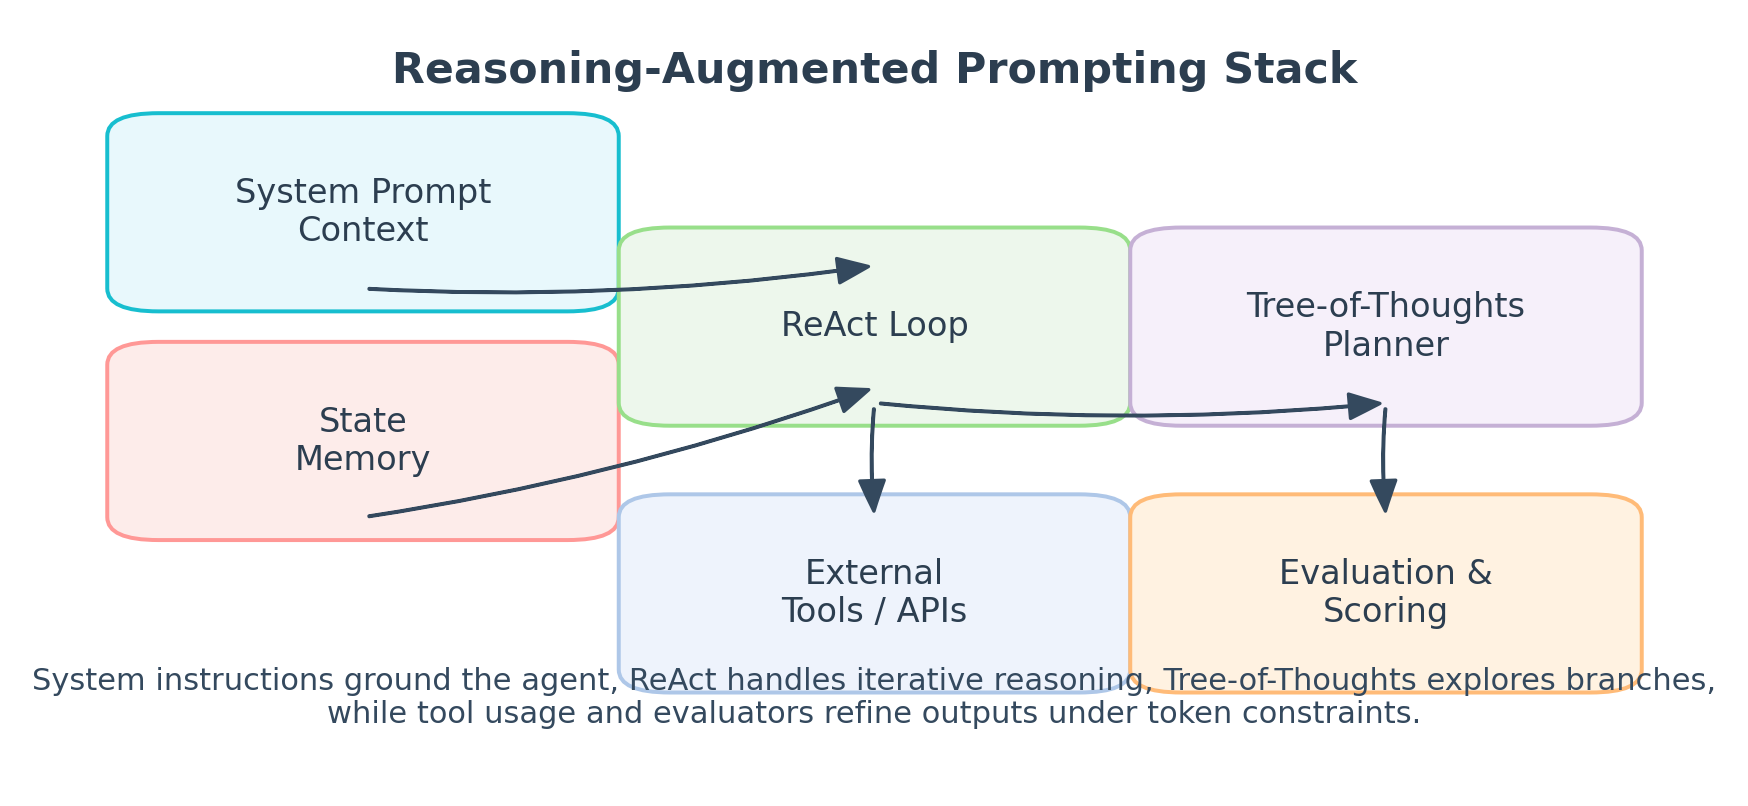
\includegraphics[width=0.92\textwidth]{reasoning_stacks.png}
  \caption{Reasoning-augmented prompting stack combining system instructions, ReAct loops, Tree-of-Thoughts exploration, tool invocation, and evaluators.}
  \label{fig:reasoning_stack_en}
\end{figure}

\section{System Prompts, Context Windows, and Token Limits}
\subsection{Designing system prompts}
System prompts define persona, tone, compliance, and overall operating rules:
\begin{itemize}
  \item \textbf{Persona framing:} State expertise, scope, and prohibited behaviors (“You are an experienced medical reviewer; you must refuse speculative diagnoses.”).
  \item \textbf{Output schema:} Specify language, formatting, and required fields to enforce consistent downstream parsing.
  \item \textbf{Safety clauses:} Reference policy documents, refusal guidance, and escalation pathways.
\end{itemize}
Complex agents may chain multiple system prompts (safety → domain → task-specific) to compose behavior.

\subsection{Managing context windows}
The context window bounds how many tokens fit in a single request/response exchange. Strategies:
\begin{itemize}
  \item \textbf{Segmentation \& summarization:} Compress stale conversation history into bullet summaries or embeddings.
  \item \textbf{Retrieval augmentation:} Store documents externally and fetch relevant passages per query, rather than injecting everything.
  \item \textbf{Sliding windows:} Drop low-priority messages as new turns arrive, preserving the most relevant few-shot examples.
  \item \textbf{Structured messages:} Use JSON/Markdown wrappers around content to facilitate automated truncation or filtering.
\end{itemize}

\subsection{Token budgeting}
Maintaining a token budget prevents latency spikes and cost overruns:
\begin{itemize}
  \item \textbf{Budget ledger:} Allocate token quotas for system prompts, user content, retrieved documents, and model output.
  \item \textbf{Estimation tools:} Run \texttt{tiktoken}, \texttt{transformers} tokenizers, or server-side accounting to measure usage ahead of time.
  \item \textbf{Degradation plans:} If usage exceeds thresholds, trigger fallbacks (summaries, shorter formats, or answer refusal).
\end{itemize}
\begin{longtable}{p{3.2cm}p{3.2cm}p{4cm}p{4cm}}
\toprule
Component & Typical length & Optimization tactic & Risk if unmanaged \\
\midrule
System prompt & 200--600 tokens & Modularize sections, reuse templates & Overlaps core content, increases latency \\
Few-shot exemplars & 50--200 tokens each & Curate representative cases, compress outputs & Context overflow leading to truncated requests \\
Retrieved docs & 200--2000 tokens & Top-$k$ filtering, summarization, reranking & Noise overwhelms the model, hallucinated answers \\
Model output & 100--800 tokens & Enforce maximum lengths, templated responses & Cut-off answers, unbounded verbosity \\
\bottomrule
\end{longtable}

\section{Prompt Optimization and Auto-Generation}
\subsection{Manual optimization loop}
\begin{enumerate}
  \item \textbf{Define success:} Establish metrics for accuracy, refusal rate, latency, and human ratings.
  \item \textbf{Baseline evaluation:} Collect canonical test prompts and expected outputs, run regression checks.
  \item \textbf{Iterative refinement:} Perform A/B testing on prompt variants, adjusting wording, examples, or structure.
  \item \textbf{Version control:} Track prompt templates, evaluation results, and rationale in Git or experiment trackers.
\end{enumerate}

\subsection{Automation techniques}
\begin{itemize}
  \item \textbf{Prompt/Prefix tuning:} Learn continuous prompt vectors appended to inputs via gradient descent.
  \item \textbf{Black-box search:} Apply genetic algorithms, Bayesian optimization, or reinforcement learning over discrete prompts.
  \item \textbf{Self-refinement:} Let the LLM critique its own prompt and propose improvements, then evaluate automatically.
  \item \textbf{Prompt compression:} Distill long prompts into concise forms via sentence selection or student models.
\end{itemize}

\subsection{Example: self-refining prompts}
\begin{lstlisting}[language=Python,caption={LLM-driven prompt refinement with self-feedback}]
import json
from transformers import AutoModelForSeq2SeqLM, AutoTokenizer

model_name = "google/flan-t5-xxl"
tokenizer = AutoTokenizer.from_pretrained(model_name)
model = AutoModelForSeq2SeqLM.from_pretrained(model_name, device_map="auto")

seed_prompt = """You are an AI assistant. Provide concise, evidence-based product comparisons."""

feedback_template = """
Original prompt:
{prompt}

Feedback questions:
1. Identify ambiguities or missing constraints.
2. Recommend improvements to clarify scope and output.
3. Suggest formatting guidance.
"""

inputs = tokenizer(feedback_template.format(prompt=seed_prompt), return_tensors="pt").to(model.device)
feedback_ids = model.generate(**inputs, max_new_tokens=256)
feedback = tokenizer.decode(feedback_ids[0], skip_special_tokens=True)

refine_template = """
Original prompt: {prompt}
Feedback: {feedback}

Produce an improved prompt that addresses the feedback and aims for higher-quality responses.
"""

inputs = tokenizer(refine_template.format(prompt=seed_prompt, feedback=feedback), return_tensors="pt").to(model.device)
refined_ids = model.generate(**inputs, max_new_tokens=160)
refined_prompt = tokenizer.decode(refined_ids[0], skip_special_tokens=True)

print(json.dumps({"feedback": feedback, "refined_prompt": refined_prompt}, indent=2))
\end{lstlisting}
Pair self-refinement with offline evaluation suites or human review to filter low-quality prompt candidates before deploying them.

\section*{Operational recommendations}
\begin{itemize}
  \item Maintain a prompt registry with consistent naming, metadata, and approval workflows across products.
  \item Combine offline evaluation datasets with online instrumentation to quantify business impact of prompt changes.
  \item Apply retrieval and summarization to conserve context window space in long-running conversations.
  \item Review automatically generated prompts for bias, policy violations, and security issues prior to rollout.
\end{itemize}

\section*{Further reading}
\begin{itemize}
  \item Wei et al. ``Chain-of-Thought Prompting Elicits Reasoning in Large Language Models.'' NeurIPS, 2022.
  \item Yao et al. ``ReAct: Synergizing Reasoning and Acting in Language Models.'' ICLR, 2023.
  \item Yao et al. ``Tree of Thoughts: Deliberate Problem Solving with Large Language Models.'' arXiv, 2023.
  \item Zhou et al. ``Large Language Models Are Human-Level Prompt Engineers.'' arXiv, 2022.
  \item Kojima et al. ``Large Language Models are Zero-Shot Reasoners.'' NeurIPS, 2022.
\end{itemize}

\end{document}

